\documentclass[dvisvgm,tikz]{standalone}

\usepackage[sfdefault]{inter}
\usetikzlibrary{shapes.geometric, arrows.meta, positioning, calc, fit, decorations.pathmorphing}

%%%%%%%%%%%%%%%%%%%%%%%%%%%%%%%%%%%%%%%%%%%%%%%%%%%
%Colors
% Warm gray to turquoise
\definecolor{warm_gray}{RGB}{128, 120, 115}
\definecolor{sage_gray}{RGB}{110, 125, 120}
\definecolor{pewter}{RGB}{91, 112, 114}
\definecolor{slate_blue}{RGB}{72, 107, 115}
\definecolor{steel_teal}{RGB}{53, 118, 125}
\definecolor{teal}{RGB}{27, 136, 140}
\definecolor{deep_aqua}{RGB}{15, 152, 155}
\definecolor{peacock_blue}{RGB}{0, 167, 171}
\definecolor{blue_green}{RGB}{0, 181, 185}
\definecolor{turquoise}{RGB}{0, 195, 200}

\definecolor{mygray}{gray}{0.9}

% Match our established color scheme
\definecolor{atoken}{RGB}{255, 152, 0}        % Orange for A token
\definecolor{gtoken}{RGB}{76, 175, 80}        % Green for G token
\definecolor{mainblue}{RGB}{74, 144, 226}     % Blue for A classes
\definecolor{maingreen}{RGB}{102, 187, 106}   % Light green for G classes
\definecolor{timegray}{RGB}{158, 158, 158}    % Gray for time component
%%%%%%%%%%%%%%%%%%%%%%%%%%%%%%%%%%%%%%%%%%%%%%%%%%%

\def \G {\textbf{G}}
\def \A {\textbf{A}}
\def \Q {\textbf{Q}}
\def \C {\textbf{C}}
\def \CC {\textbf{C*}}
\def \KA {\textbf{KLIMA}}
\def \KG {\textbf{KlimaX}}

\def \AG {$\overline{\textbf{AG}}$}
\def \AQ {$\overline{\textbf{AQ}}$}

\begin{document}
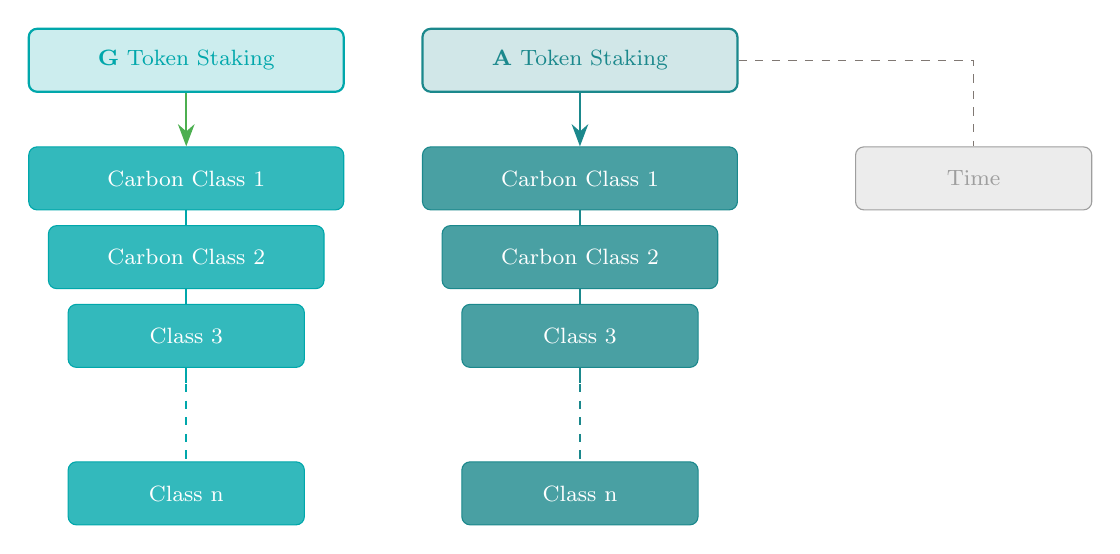
\begin{tikzpicture}[
    token/.style={
        rectangle,
        draw=#1,
        fill=#1!20,
        thick,
        minimum width=4cm,
        minimum height=0.8cm,
        text=#1,
        align=center,
        rounded corners=3pt,
        font=\footnotesize
    },
    class/.style={
        rectangle,
        draw=#1,
        fill=#1!80,
        text=white,
        minimum height=0.8cm,
        align=center,
        rounded corners=3pt,
         font=\footnotesize
    },
    time/.style={
        rectangle,
        draw=timegray,
        fill=timegray!20,
        text=timegray,
        minimum width=3cm,
        minimum height=0.8cm,
        align=center,
        rounded corners=3pt,
        font=\footnotesize
    },
    arrow/.style={
        -{Stealth[length=8pt]},
        thick,
        #1
    }
]

% Define column positions
\def\colA{-5}    % G Token column
\def\colB{0}     % A Token column
\def\colC{5}     % Time column

% Token staking nodes at the top
\node[token=peacock_blue] (gstaking) at (\colA,4) {\G{} Token Staking};
\node[token=teal] (astaking) at (\colB,4) {\A{} Token Staking};

% Classes for G token with consistent widths
\node[class=peacock_blue, minimum width=4cm] (g1) at (\colA,2.5) {Carbon Class 1};
\node[class=peacock_blue, minimum width=3.5cm] (g2) at (\colA,1.5) {Carbon Class 2};
\node[class=peacock_blue, minimum width=3cm] (g3) at (\colA,0.5) {Class 3};
\node[class=peacock_blue, minimum width=3cm] (gn) at (\colA,-1.5) {Class n};

% Classes for A token aligned with G token classes
\node[class=teal, minimum width=4cm] (a1) at (\colB,2.5) {Carbon Class 1};
\node[class=teal, minimum width=3.5cm] (a2) at (\colB,1.5) {Carbon Class 2};
\node[class=teal, minimum width=3cm] (a3) at (\colB,0.5) {Class 3};
\node[class=teal, minimum width=3cm] (an) at (\colB,-1.5) {Class n};

% Time component aligned with first class level
\node[time] (time) at (\colC,2.5) {Time};

% Connecting arrows - now from center to center
\draw[arrow=gtoken] (gstaking.south) -- (g1.north);
% Split A token arrows from the same point
\coordinate[below=0.4cm of astaking] (split) at (astaking.south);
\draw[arrow=teal] (astaking.south) -- (a1.north);
\draw[dashed,warm_gray] (astaking.east) -| (time.north);

% Vertical connections between classes
\foreach \y in {2.5,1.5,0.5} {
    \pgfmathsetmacro{\nexty}{\y-1}
    \draw[thick, peacock_blue] (\colA,\y-0.4) -- (\colA,\nexty+0.4);
    \draw[thick, teal] (\colB,\y-0.4) -- (\colB,\nexty+0.4);
}

% Dashed lines to indicate continuation
\draw[dashed, peacock_blue, thick] (\colA,0.1) -- (\colA,-1.1);
\draw[dashed, teal, thick] (\colB,0.1) -- (\colB,-1.1);

\end{tikzpicture}
\end{document}
